\paragraph{Base64}

All the materials shown in MathChatBot are made using LaTeX. The Snipping Tool in Windows has been used to separate each definition, example and assignment. The images are then stored in the database using Base64 encoding. An alternative would be compiling the images from LaTeX. There are no existing libraries in C\# that can compile the images from LaTeX. Therefore the only other option left would be to do the conversion via an external program such as MiKTeX. The problem with using MiKTeX is the fact that every user would have to download the program onto their computer which was deemed to be to bothersome and ineffective. Another option was creating a file table for the MathChatBot which could have been taken in use for storing the images, this option has not been pursued since setting up the whole file table would have taken to much of the time dedicated to this project. Because using MiKTeX was deemed to bothersome and creating a filetable would have taken too much time the MathChatBot makes use of Base64 encoding, this being said a library with the same features as MiKTeX would have been the most effective solution with the time limit set on this project. Base64 is a process of converting any form of data from binary data into a 6-bit character representation and then converting the 6-bit character representation using the Base64 encoding table. This process can also be seen on \figureref{fig:base64_encoding}.

\begin{figure}[H]
    \centering
    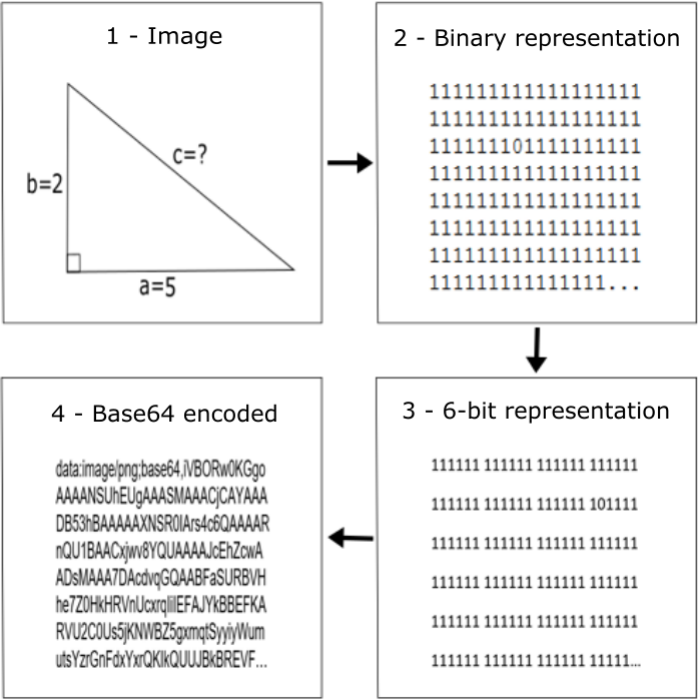
\includegraphics[width=0.6\textwidth]{figures/image1412.png}
    \caption{The steps of Base64 encoding \cite{DemoAPI}}
    \label{fig:base64_encoding}
\end{figure}

\noindent
One part number one of \figureref{fig:base64_encoding} the original image is depicted that is going to be Base64 encoded. In step number 2 the image is converted into binary form. For the assignments, examples and definitions used for the MathChatBot mostly black and white images are used, which makes the conversion to binary much less extensive. every number 1 in the binary representation represents a white pixel while every 0 represents a black pixel. Colored images will take up more space since the number of colors increases and therefore the complexity of the binary conversion also increases. The full binary representation of the image on \figureref{fig:base64_encoding} is still too extensive to be put into \figureref{fig:base64_encoding} therefore only a small portion of the binary representation has been used. The next step of a Base64 encoding is separating the binary representation into sets of 6 bits. This is done due to some issues with sending binary data across a network, transferring the raw bytes may not be a good option as some media are made for streaming text. Some protocols may interpret your binary data as control characters which will result in the data getting corrupted. Since Base64 conversion uses a 6-bit representation it has 64 characters available, this is also where it has its name from. These characters include the numbers from 0-9, 26 lowercase letters and 26 uppercase letters as well as the plus sign and the forward slash. Furthermore there is also at 65th character known as a pad which is represented with the equals sign. This is used when the last part of the binary representation does not contain a full 6 bits. For the last step the Base64 encoding table is used where every 6 bits are converted into a character\cite{HeinzTschabitscher2019HowWorks}.

